% Make clear about using the window function in the frequency domain as a filter.
%%%%%%%%%%%%%%%%%%%%%%%%%%%%%%%%%
\newpage
%%%%%%%%%%%%%%%%%%%%%%%%%%%%%%%%%
\section{The transition to the Fourier Transform}

\subsection*{Resources}
\begin{itemize}
    \item Video I: Lecture 5 from 27:00 (\url{https://youtu.be/X5qRpgfQld4?t=27m})
    \item Video II: Lecture 6 up to 20:00 (\url{https://www.youtube.com/watch?v=4lcvROAtN_Q})
    \item Book: Chapter 2 (\url{https://see.stanford.edu/materials/lsoftaee261/book-fall-07.pdf})
\end{itemize}

\subsection*{Comment}
Until now we have been considering Fourier series. This is however limited to describing periodic phenomena since it is assumed that the signal repeats outside the region of integration. The Fourier transform can be thought of as an extension of Fourier series which allows the analysis of non-periodic phenomena.

The suggested resources provide an excellent intuitive path of the connection between Fourier series and Fourier transforms, and this challenge is designed to give you the opportunity to take some time to try to understand the main concepts behind the transition.

\subsection*{Challenge}
Using the resources above, describe how to make the transition from Fourier series to the Fourier transform.



%%%%%%%%%%%%%%%%%%%%%%%%%%%%%%%%%
\newpage
%%%%%%%%%%%%%%%%%%%%%%%%%%%%%%%%%
\section{Fourier transform notation}

\subsection*{Comment}
Just so that you are aware, you should know that there are various equivalent notations in use, and if you use the Fourier transform in your later career you will probably come across notations different to the ones used in this course. This is partly because Fourier analysis is applicable to a wide range of fields and each field tends to have its own conventions based on how the Fourier transform is interpreted physically (if at all) in that field.

In general, the Fourier transform is given by
\begin{equation}
    \mathcal{F}f(\omega) = \sqrt{\frac{|b|}{(2 \pi)^{1-a}}} \int_{-\infty}^{\infty} f(t) e^{i b \omega t} dt
\end{equation}

where $a$ and $b$ typically take on values such as 

\begin{tabular}{|c|c c|}
    \hline
    \textbf{Case} & \textbf{a} & \textbf{b} \\
    \hline
    \textbf{1}    & 0          & 1          \\
    \textbf{2}    & 1          & -1         \\
    \textbf{3}    & -1         & 1          \\
    \textbf{4}    & 0          & -2$\pi$   \\
    \hline
\end{tabular}

\subsection*{Challenge}
1. Write the Fourier transform using the four possible notations.

2. Add the points of the legitimate forms of Fourier notation:

1 point: $\displaystyle \mathcal{F}f(w)=\frac{1}{\sqrt{2 \pi}} \int_{-\infty}^{\infty} e^{i w t} f(t) dt$

2 points: $\displaystyle \mathcal{F}f(w)=\int_{-\infty}^{\infty} e^{-i 2 \pi w t} f(t) dt$

4 points: $\displaystyle \mathcal{F}f(w)=\frac{1}{2 \pi} \int_{-\infty}^{\infty} e^{i w t} f(t) dt$

8 points: $\displaystyle \mathcal{F}f(s)=\frac{1}{\sqrt{2 \pi}} \int_{-\infty}^{\infty} e^{i \pi s t} f(t) dt$

16 points: $\displaystyle \mathcal{F}f(w)=\int_{-\infty}^{\infty} e^{i 2 \pi w t} f(t) dt$

32 points: $\displaystyle \mathcal{F}f(s)=\int_{-\infty}^{\infty} e^{-i s t} f(t) dt$

\subsection*{Solution}
2.\\
\solint{c}{8cecbb}




%%%%%%%%%%%%%%%%%%%%%%%%%%%%%%%%%
\newpage
%%%%%%%%%%%%%%%%%%%%%%%%%%%%%%%%%
\section{L'H\^opital's rule}

\subsection*{Challenge}
Use L'H\^opital's rule to determine the limit of
\begin{equation}
    \frac{\sin(x)}{x}
\end{equation}
as $x \rightarrow 0$.

\subsection*{Solution}
\solint{d}{9948c6}




%%%%%%%%%%%%%%%%%%%%%%%%%%%%%%%%%
\newpage
%%%%%%%%%%%%%%%%%%%%%%%%%%%%%%%%%
\section{Fourier transform of a window function}
\label{sec:tophat}

\subsection*{Resources}
\begin{itemize}
    \item Book: Chapter 2.1 (\url{https://see.stanford.edu/materials/lsoftaee261/book-fall-07.pdf}) %, page 68, particularly at the bottom of the page
    \item Video: Lecture 6 starting from 29:26 (\url{https://youtu.be/4lcvROAtN_Q?t=29m26s})
\end{itemize}

\subsection*{Challenge}
Calculate the Fourier Transform for the window function

\begin{equation}
    f(t)=
    \begin{cases}
        1 & \text{for } |t| < 1/2 \\
        0 & \text{for } |t| > 1/2
    \end{cases}
\end{equation}

In graph-form the function and its transform appear as follows:

\begin{tabular}{cc}
    \textbf{Function} & \textbf{Fourier transform} \\
    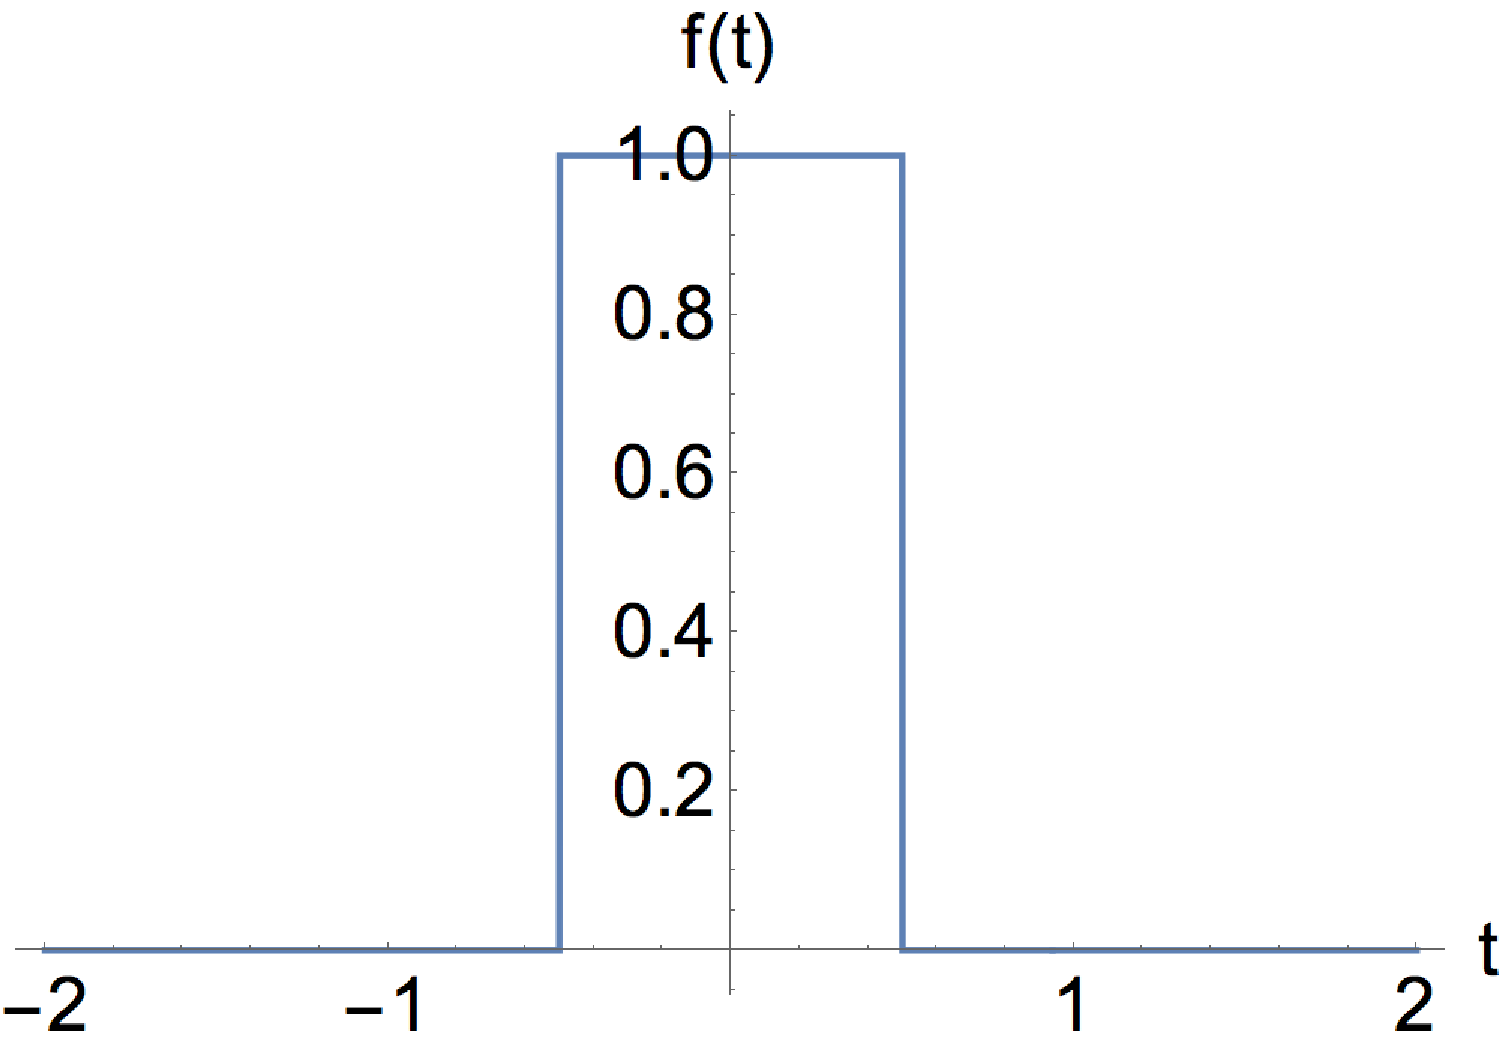
\includegraphics[scale=0.5]{window1.png} & 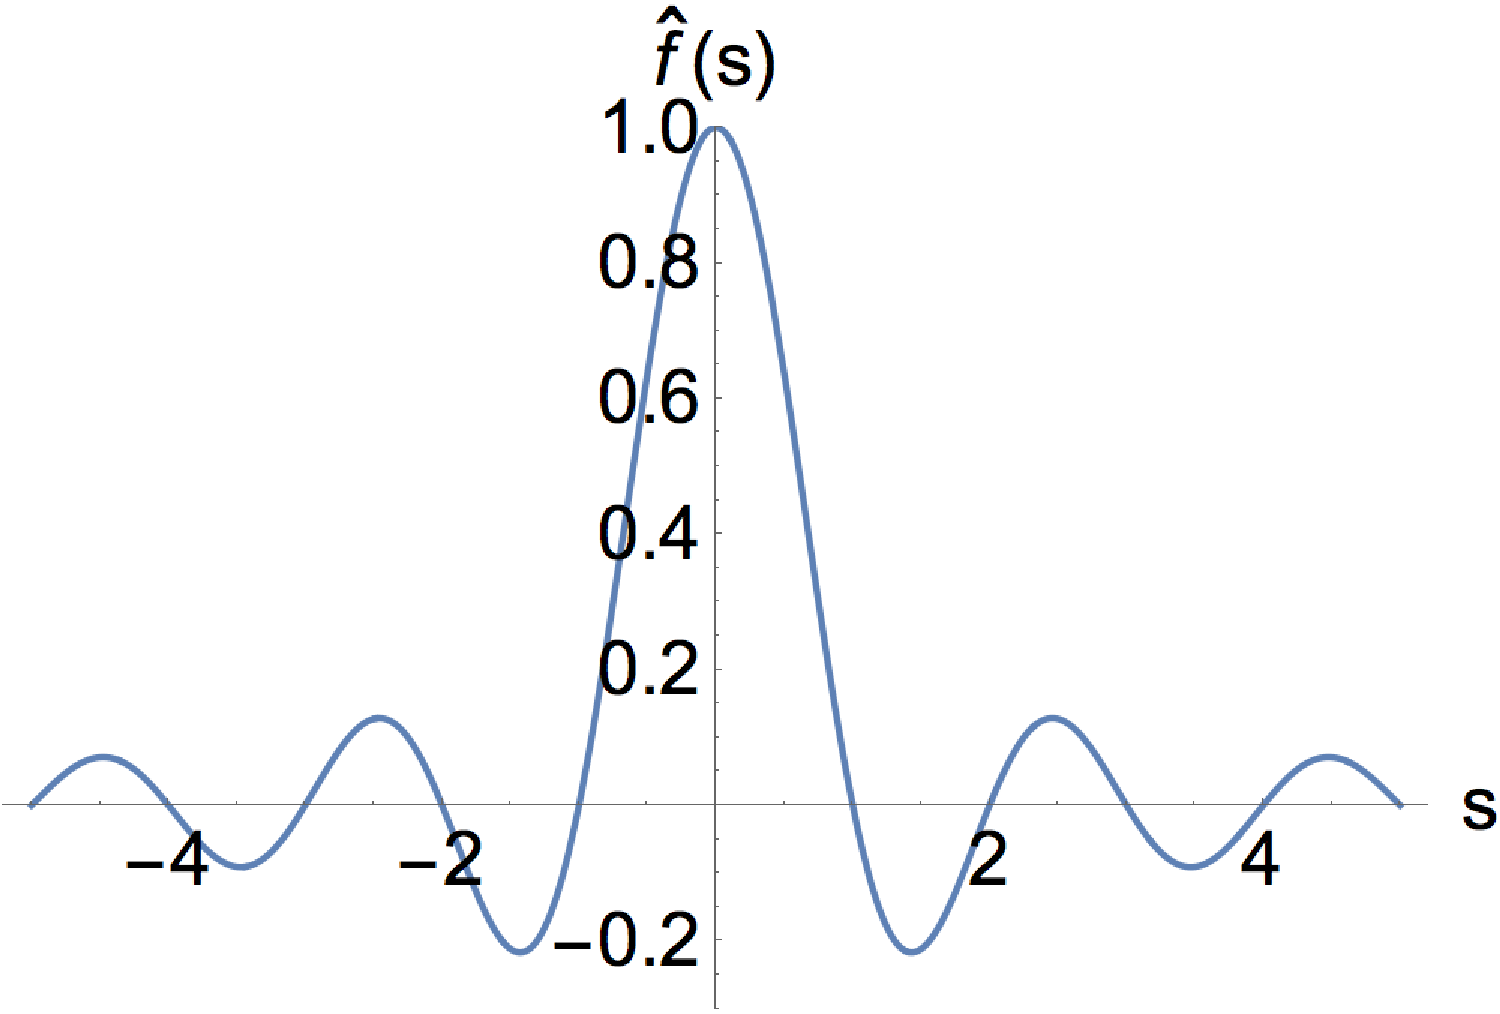
\includegraphics[scale=0.5]{window1ft.png}
\end{tabular}

\subsection*{Solution}
You should find that your solution is consistent with $\hat{f}(s=1.5)=-0.21$.




%%%%%%%%%%%%%%%%%%%%%%%%%%%%%%%%%
\newpage
%%%%%%%%%%%%%%%%%%%%%%%%%%%%%%%%%
\section{Fourier transform of sine and cosine}

\subsection*{Comments}
With Fourier series we understood the integer $k$ in $\sin(2 \pi k t)$ as the frequency of the signal, and by building up the sum of sines and cosines (using exponential notation) we could reproduce very well an arbitrary periodic signal. In the case of challenges \ref{sec:fcsinx} and \ref{sec:fcsinxp1} we determined the Fourier coefficients for a single-frequency $k=1$ sine signal.

Can we still understand the $s$ in the Fourier transform $\int_{-\infty}^{\infty} f(t) e^{i 2 \pi s t}$ as analogous to $k$ somehow? What happens when you take the Fourier transform of a single-frequency signal? How is phase-information encoded? This is difficult to visualise but this challenge, dealing with simple single-frequency signals, should give you an initial insight.

\subsection*{Challenge}
1. Calculate the Fourier transforms of\\
(I) $\sin(2 \pi t)$\\
(II) $\cos(2 \pi t)$

You may find the following identity useful:
\begin{equation}
    \int_{-\infty}^{\infty} e^{-i 2 \pi (s+c) t} = \delta(s+c)
\end{equation}

2. Write $\sin(2 \pi t)$ and $\cos(2 \pi t)$ in terms of complex exponentials. Can you see an analogy between the Fourier transforms you calculated and the complex exponential forms of sine and cosine?

\subsection*{Solution}
1. In both cases, to check your answers calculate $\int_0^2 f(s) ds$.

(I)\\
\solimagtwodp{e}{923c59}

(II)\\
\solimagtwodp{f}{c68bbf}

2. Please discuss with your partner in class, and ask the teacher if you are unsure.



%%%%%%%%%%%%%%%%%%%%%%%%%%%%%%%%%
\newpage
%%%%%%%%%%%%%%%%%%%%%%%%%%%%%%%%%
\section{Fourier transform of a triangle function}
\label{sec:ft_triangle}

\subsection*{Resources}
\begin{itemize}
    \item Book: Chapter 2.2.1 (\url{https://see.stanford.edu/materials/lsoftaee261/book-fall-07.pdf})
    \item Video: Lecture 6 (\url{https://www.youtube.com/watch?v=4lcvROAtN_Q})
\end{itemize}

\subsection*{Challenge}
What is the Fourier transform of a triangle function, as shown below, in terms of the window function of challenge \ref{sec:tophat}? You may just state the function; calculation is not required unless you would like to try and prove it.

\begin{tabular}{cc}
    \textbf{Function} & \textbf{Fourier transform} \\
    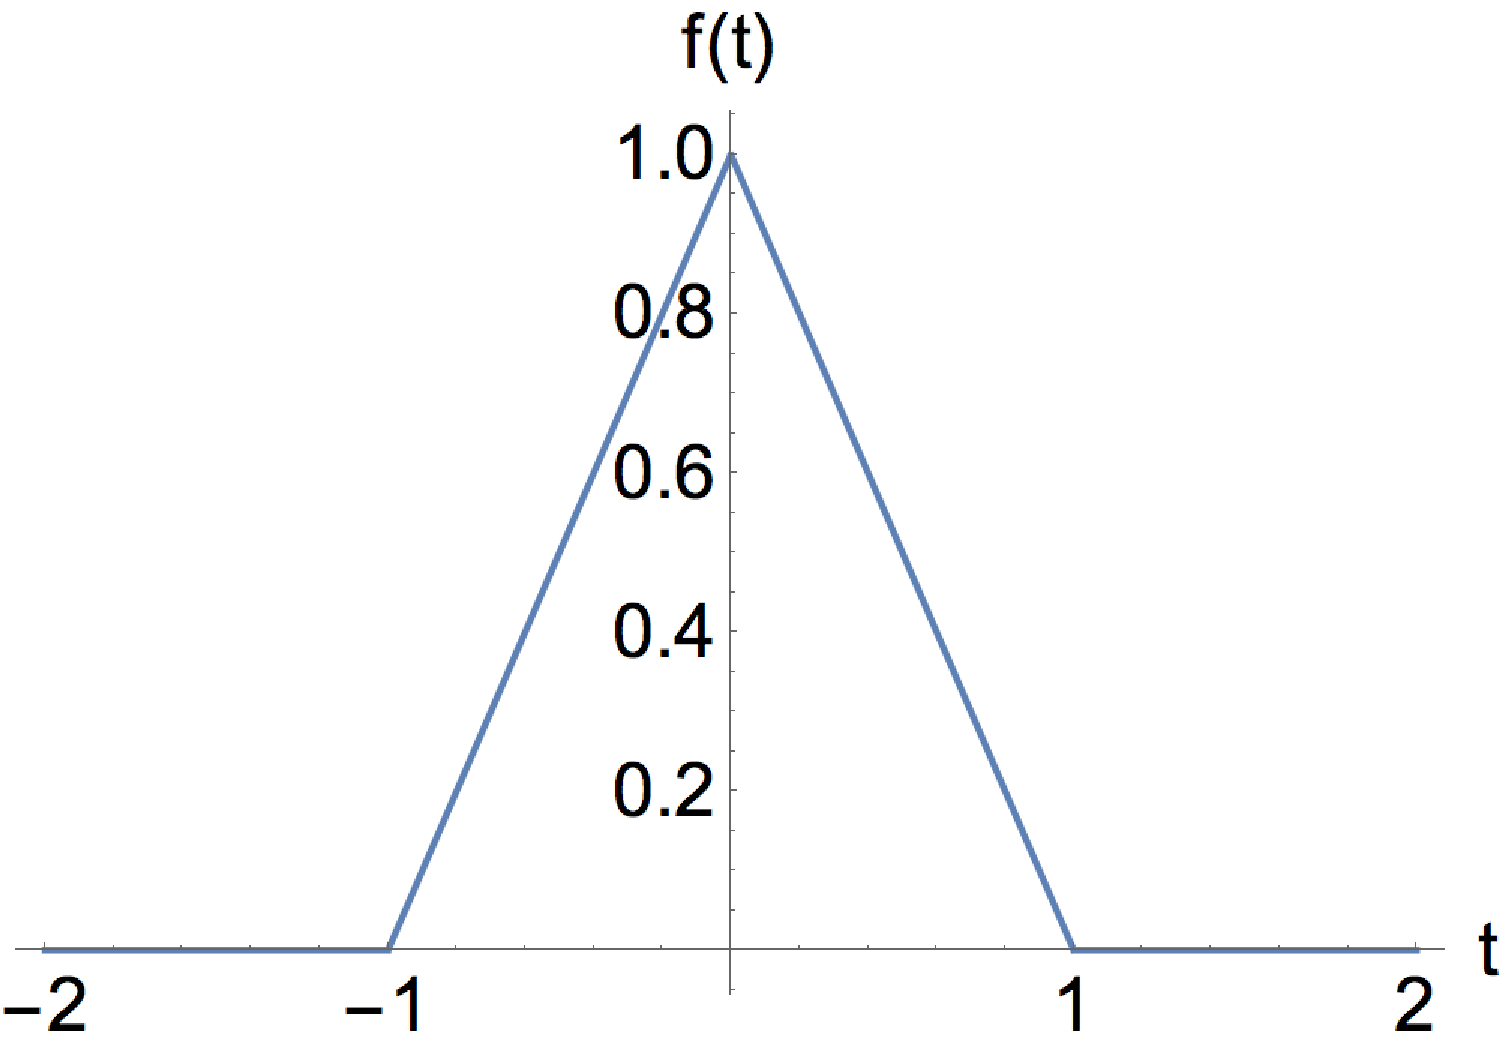
\includegraphics[scale=0.5]{triangle.png} & 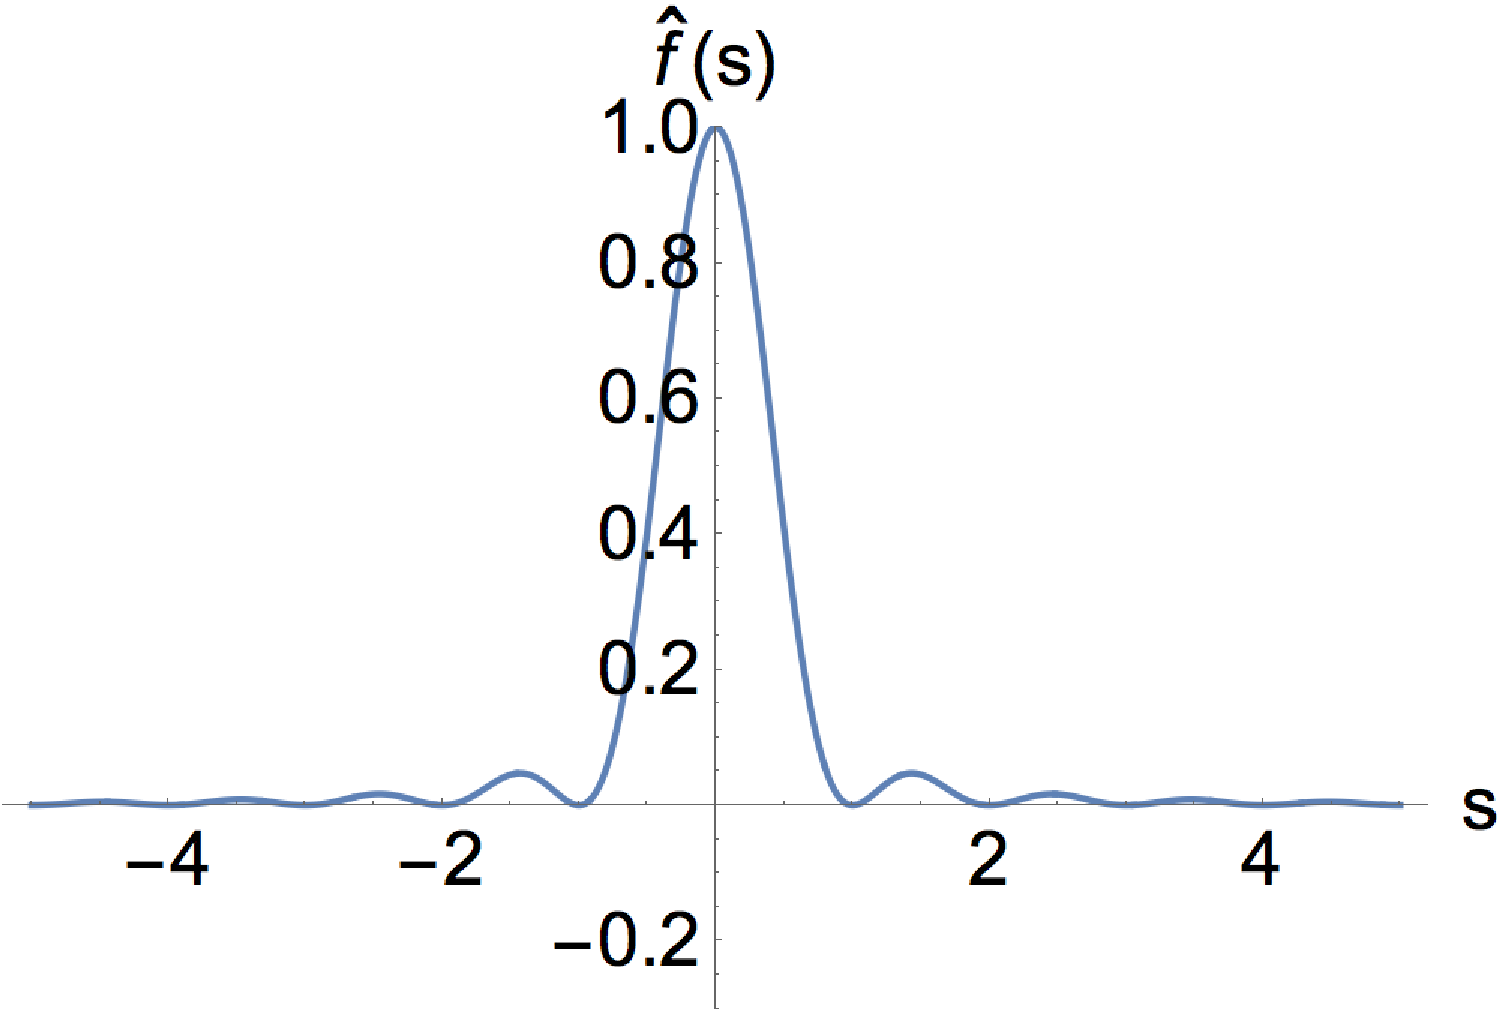
\includegraphics[scale=0.5]{triangleft.png}
\end{tabular}

\subsection*{Solution}
Your answer should be consistent with $F(s=1.5) = 0.045$




%%%%%%%%%%%%%%%%%%%%%%%%%%%%%%%%%
\newpage
%%%%%%%%%%%%%%%%%%%%%%%%%%%%%%%%%
\section{Fourier transform of a Gaussian}

\subsection*{Resources}
\begin{itemize}
    \item Book: Chapter 2.2.2 (\url{https://see.stanford.edu/materials/lsoftaee261/book-fall-07.pdf})
    \item Video: Lecture 7 (\url{https://www.youtube.com/watch?v=mdFETbe1n5Q})
\end{itemize}

\subsection*{Challenge}
Starting from the general formula for Fourier transform, calculate the Fourier transform for the Gaussian function:

\begin{equation}
    f(t) = e^{-\pi t^2}
\end{equation}

The Gaussian function looks like

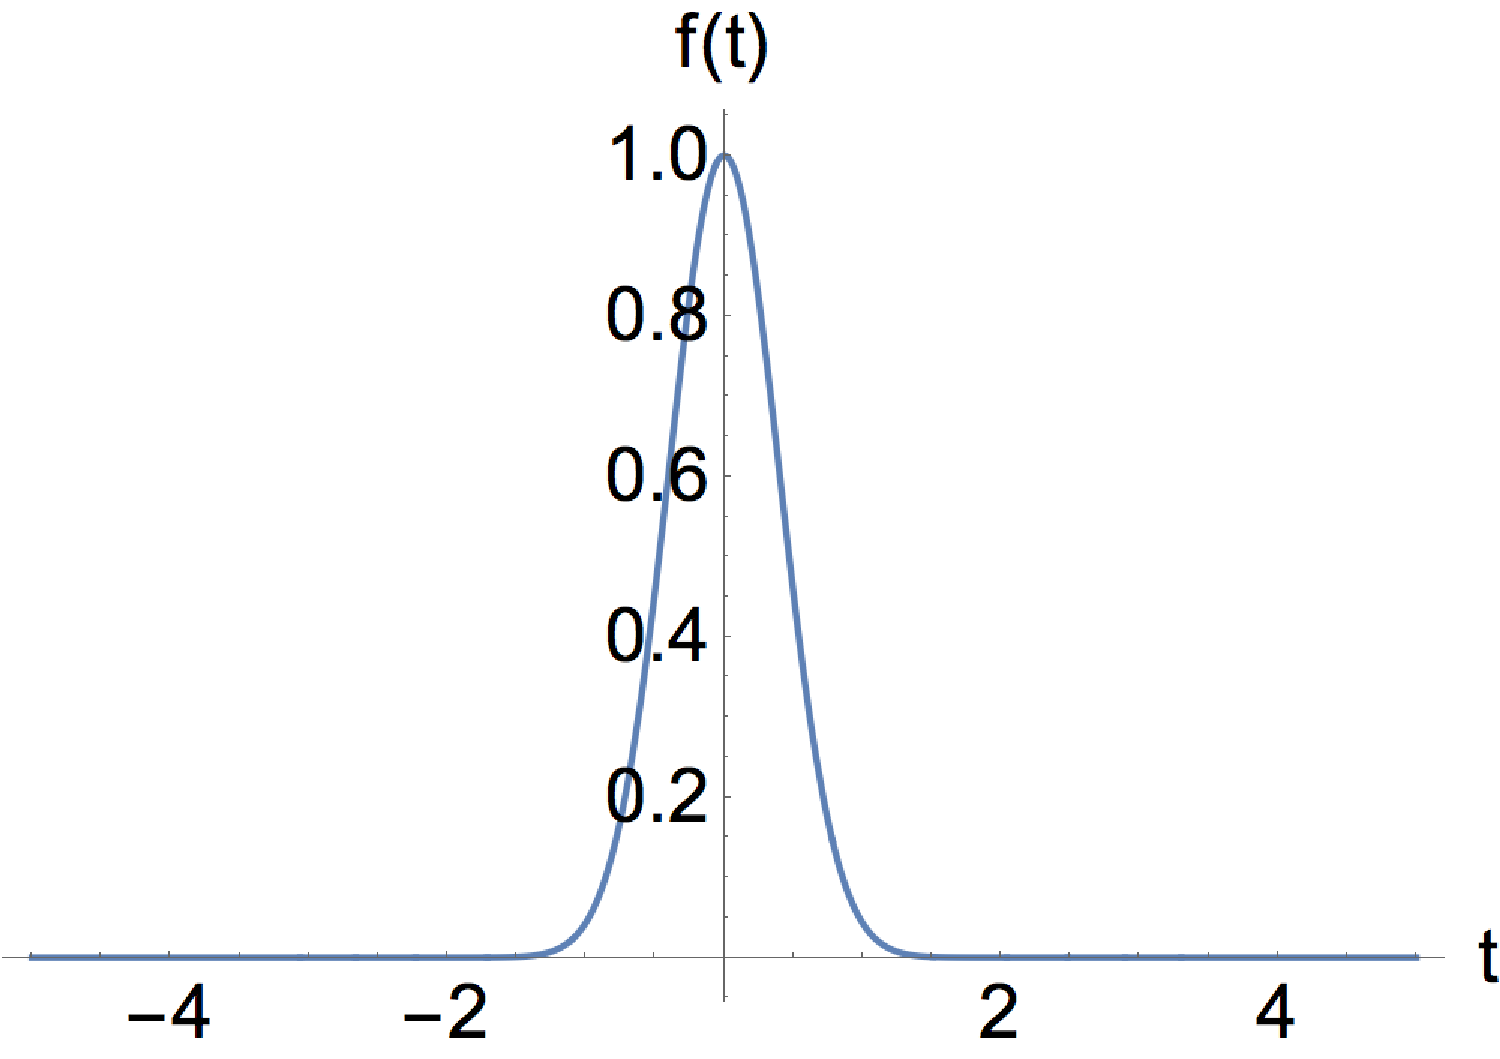
\includegraphics[width=8cm]{gaussian.png}

\subsection*{Solution}
Your answer should be consistent with $F(s=1.5) =$ \num{8.51e-4}




%%%%%%%%%%%%%%%%%%%%%%%%%%%%%%%%%
\newpage
%%%%%%%%%%%%%%%%%%%%%%%%%%%%%%%%%
\section{Fourier transform of a rocket function}

\subsection*{Resources}
\begin{itemize}
    \item Book: Chapter 2.2.6 (\url{https://see.stanford.edu/materials/lsoftaee261/book-fall-07.pdf})
\end{itemize}

\subsection*{Challenge}
Calculate the Fourier Transform for the rocket function:
\begin{equation}
    f(at)=
    \begin{cases}
        2 - |t| & \text{for } 0 \le |t| < \frac{1}{2}\\
        1 - |t| & \text{for } \frac{1}{2} \le |t| \le 1\\
        0 & \text{otherwise}
    \end{cases}
\end{equation}
    
shown below. In graph-form the function and its transform appear as follows:

\begin{tabular}{cc}
    \textbf{Function} & \textbf{Fourier transform} \\
    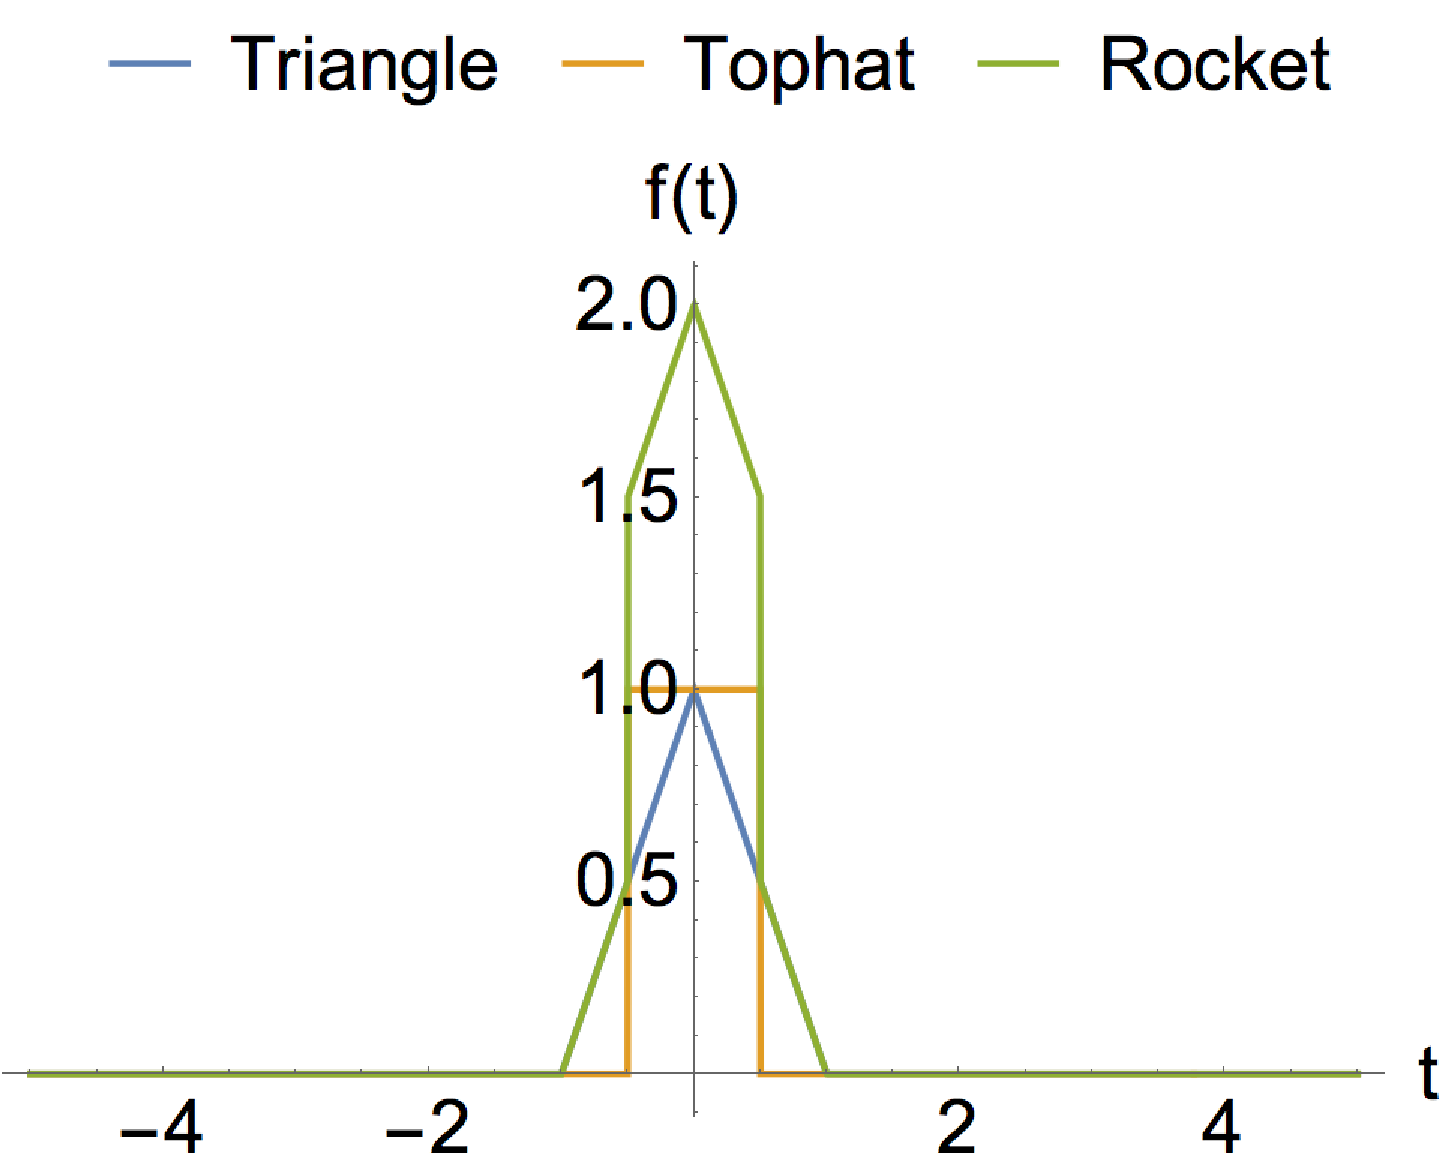
\includegraphics[scale=0.6]{rocket.png} & 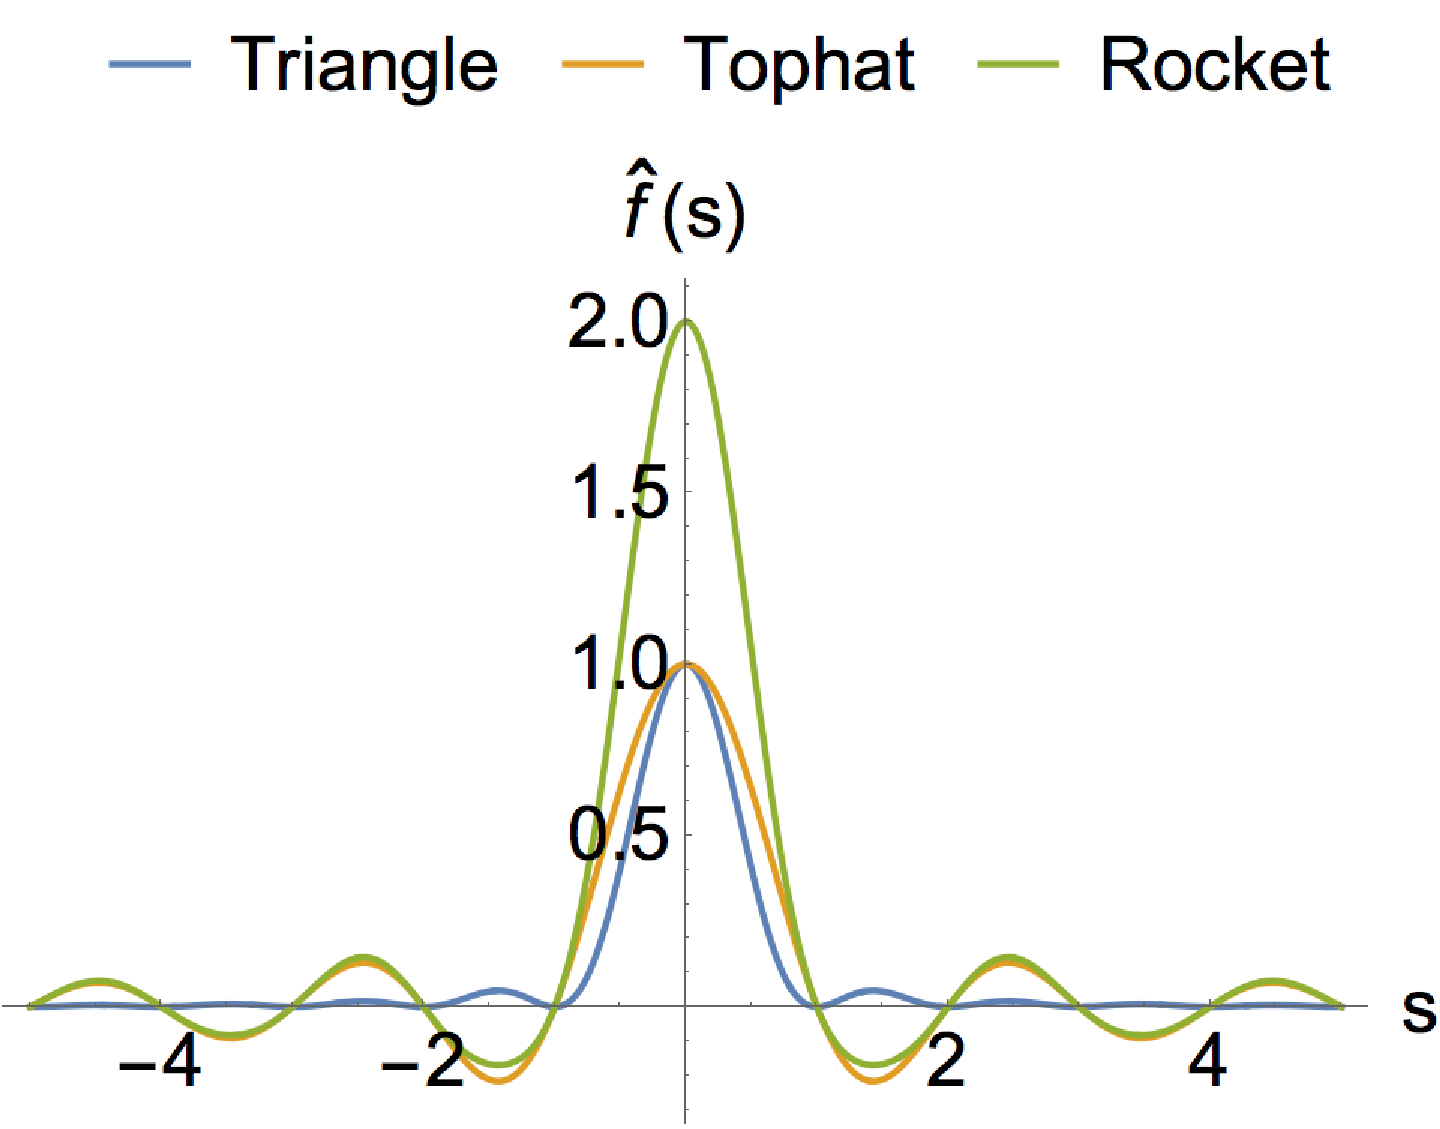
\includegraphics[scale=0.6]{rocketft.png}
\end{tabular}

\subsection*{Solution}
Your answer should be consistent with $F(s=1.5) = -0.17$




%%%%%%%%%%%%%%%%%%%%%%%%%%%%%%%%%
\newpage
%%%%%%%%%%%%%%%%%%%%%%%%%%%%%%%%%
\section{Fourier transform of a shifted window function}

\subsection*{Resources}
\begin{itemize}
    \item Book: Chapter 2.2.7 (\url{https://see.stanford.edu/materials/lsoftaee261/book-fall-07.pdf})
    \item Video lecture 8 from 1:56 to 11:20 (\url{https://youtu.be/wUT1huREHJM?t=1m56s})
\end{itemize}

\subsection*{Challenge}
1. What is meant by a ``phase-shift'' of a signal in time? What does it mean in terms of the window-function here?

2. Calculate the Fourier Transform for the window function delayed by \SI{1}{\second}.

A graph with increasing delay is shown in the figure below. What is happening to the real and imaginary parts of the signal as the delay increases? You considered the original window function in challenge \ref{sec:tophat}.

\begin{tabular}{c}
    \textbf{Function} \\
    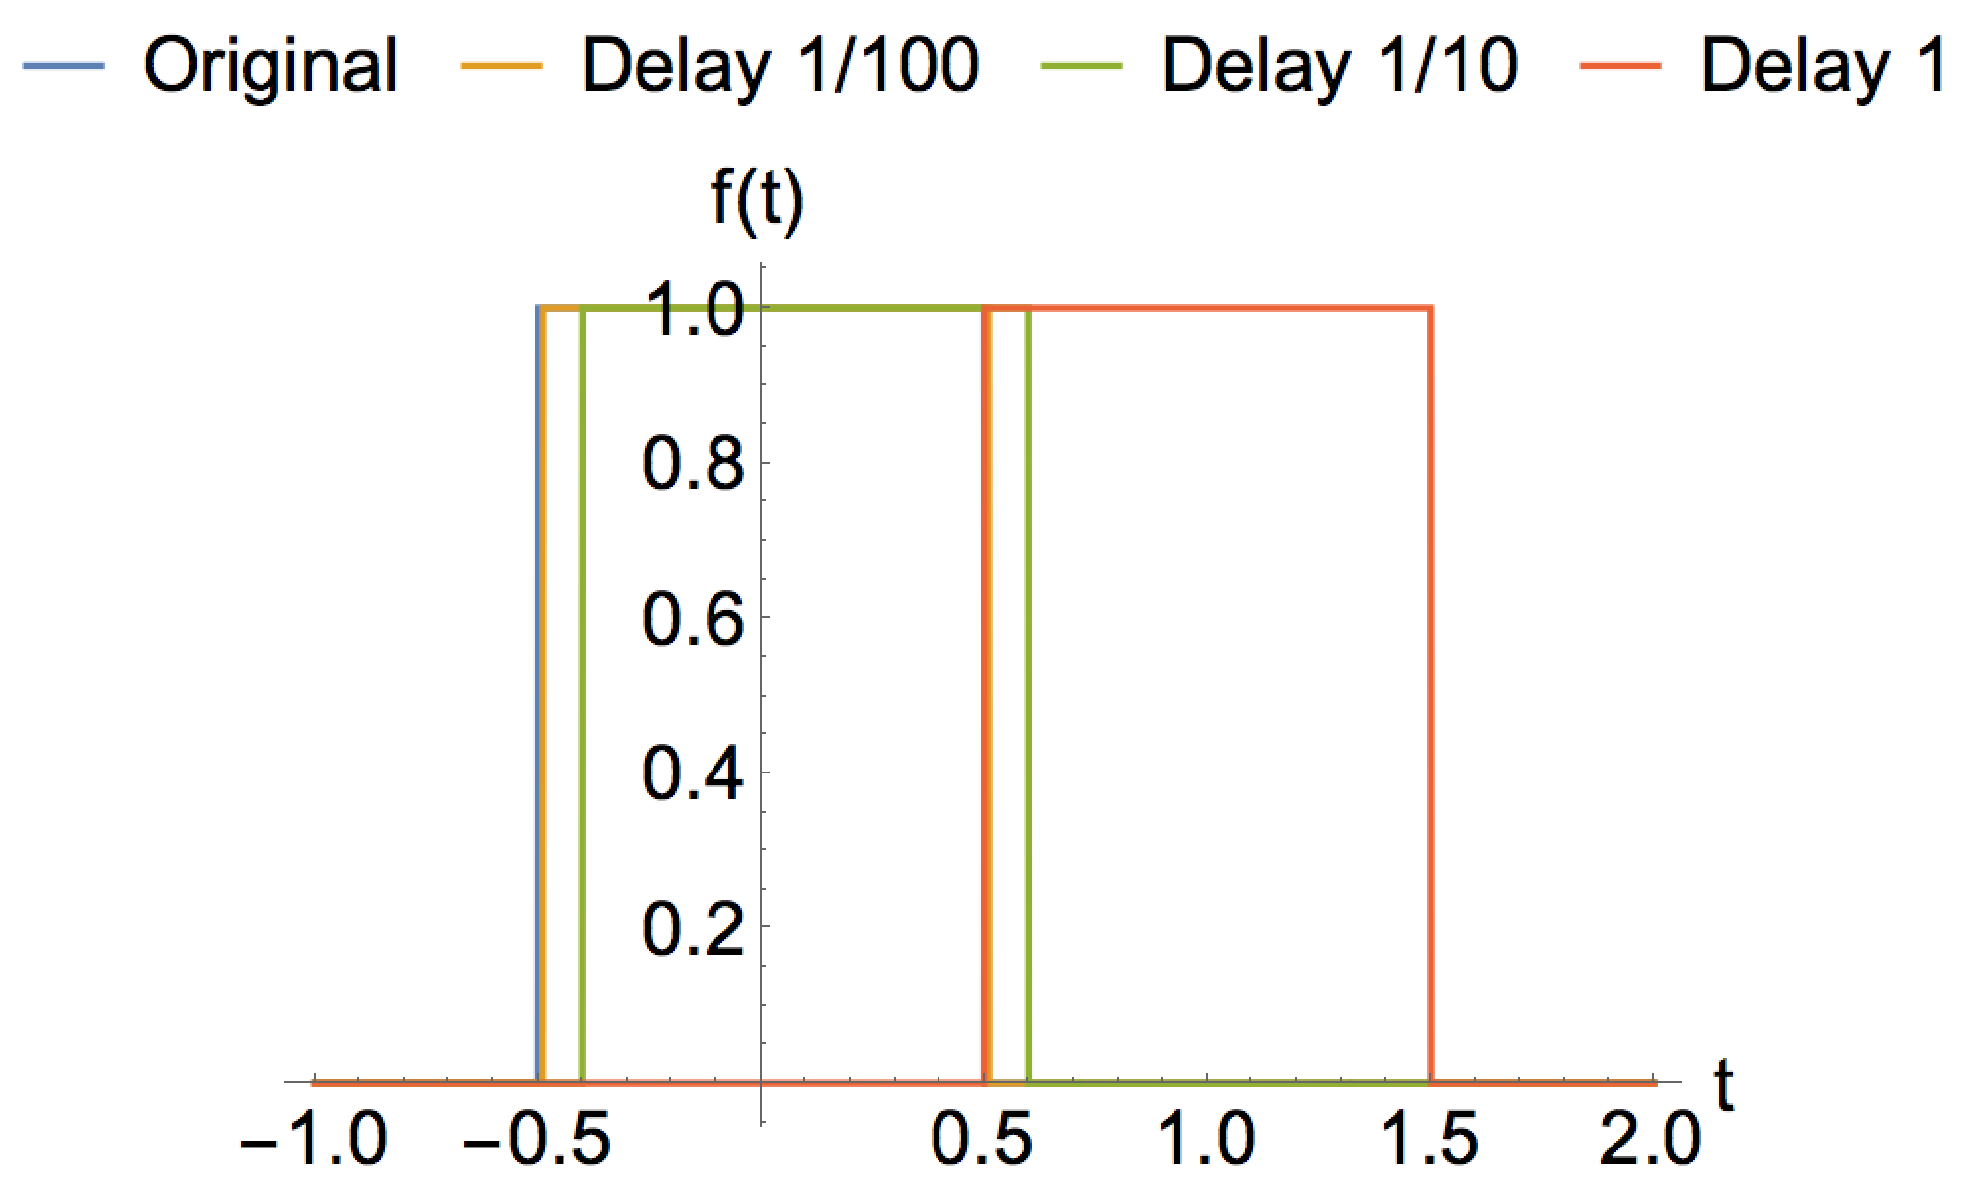
\includegraphics[scale=0.5]{tophatdelay.png}
\end{tabular}

\begin{tabular}{cc}
    \textbf{Fourier transform (real part)} & \textbf{Fourier transform (imaginary part)}\\
    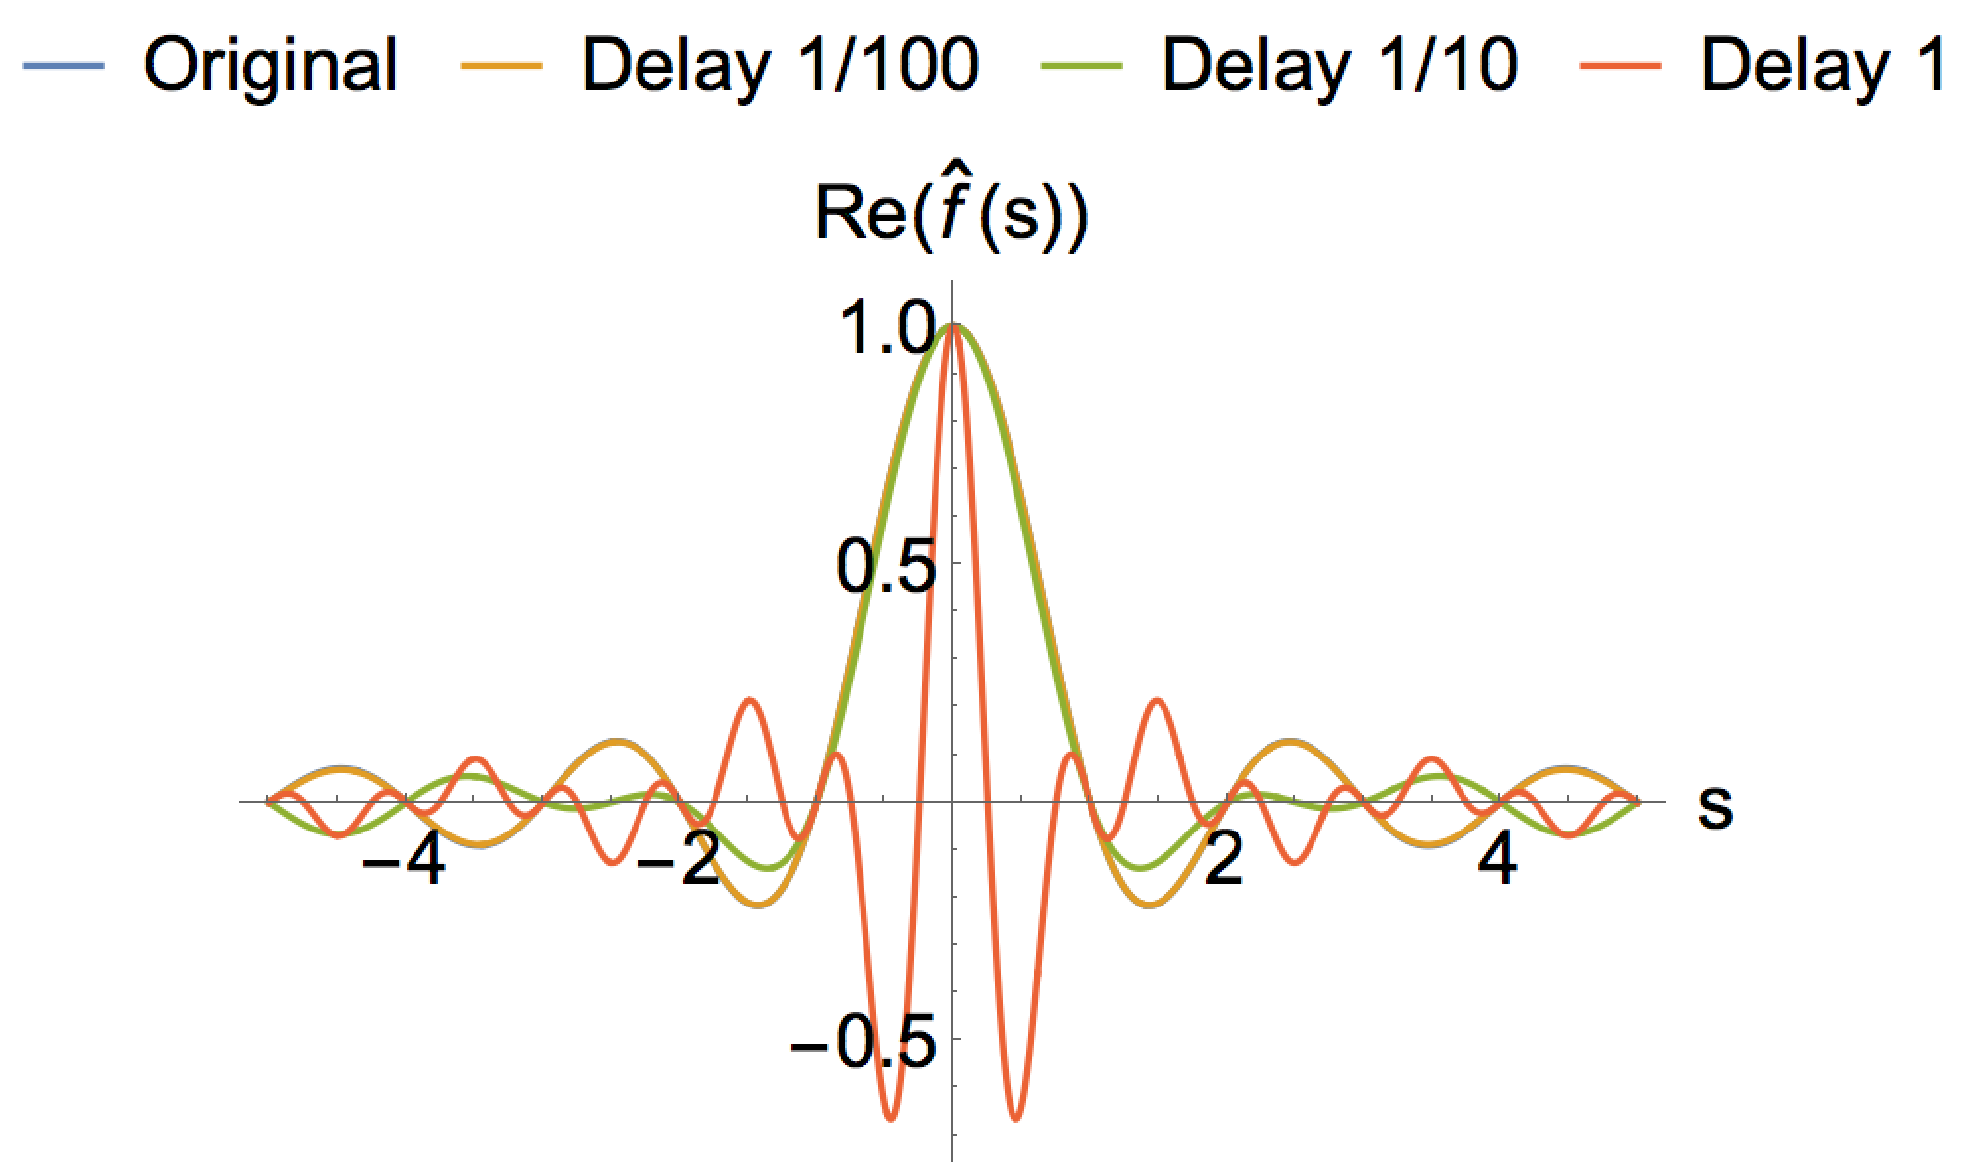
\includegraphics[scale=0.5]{tophatdelayre.png} & 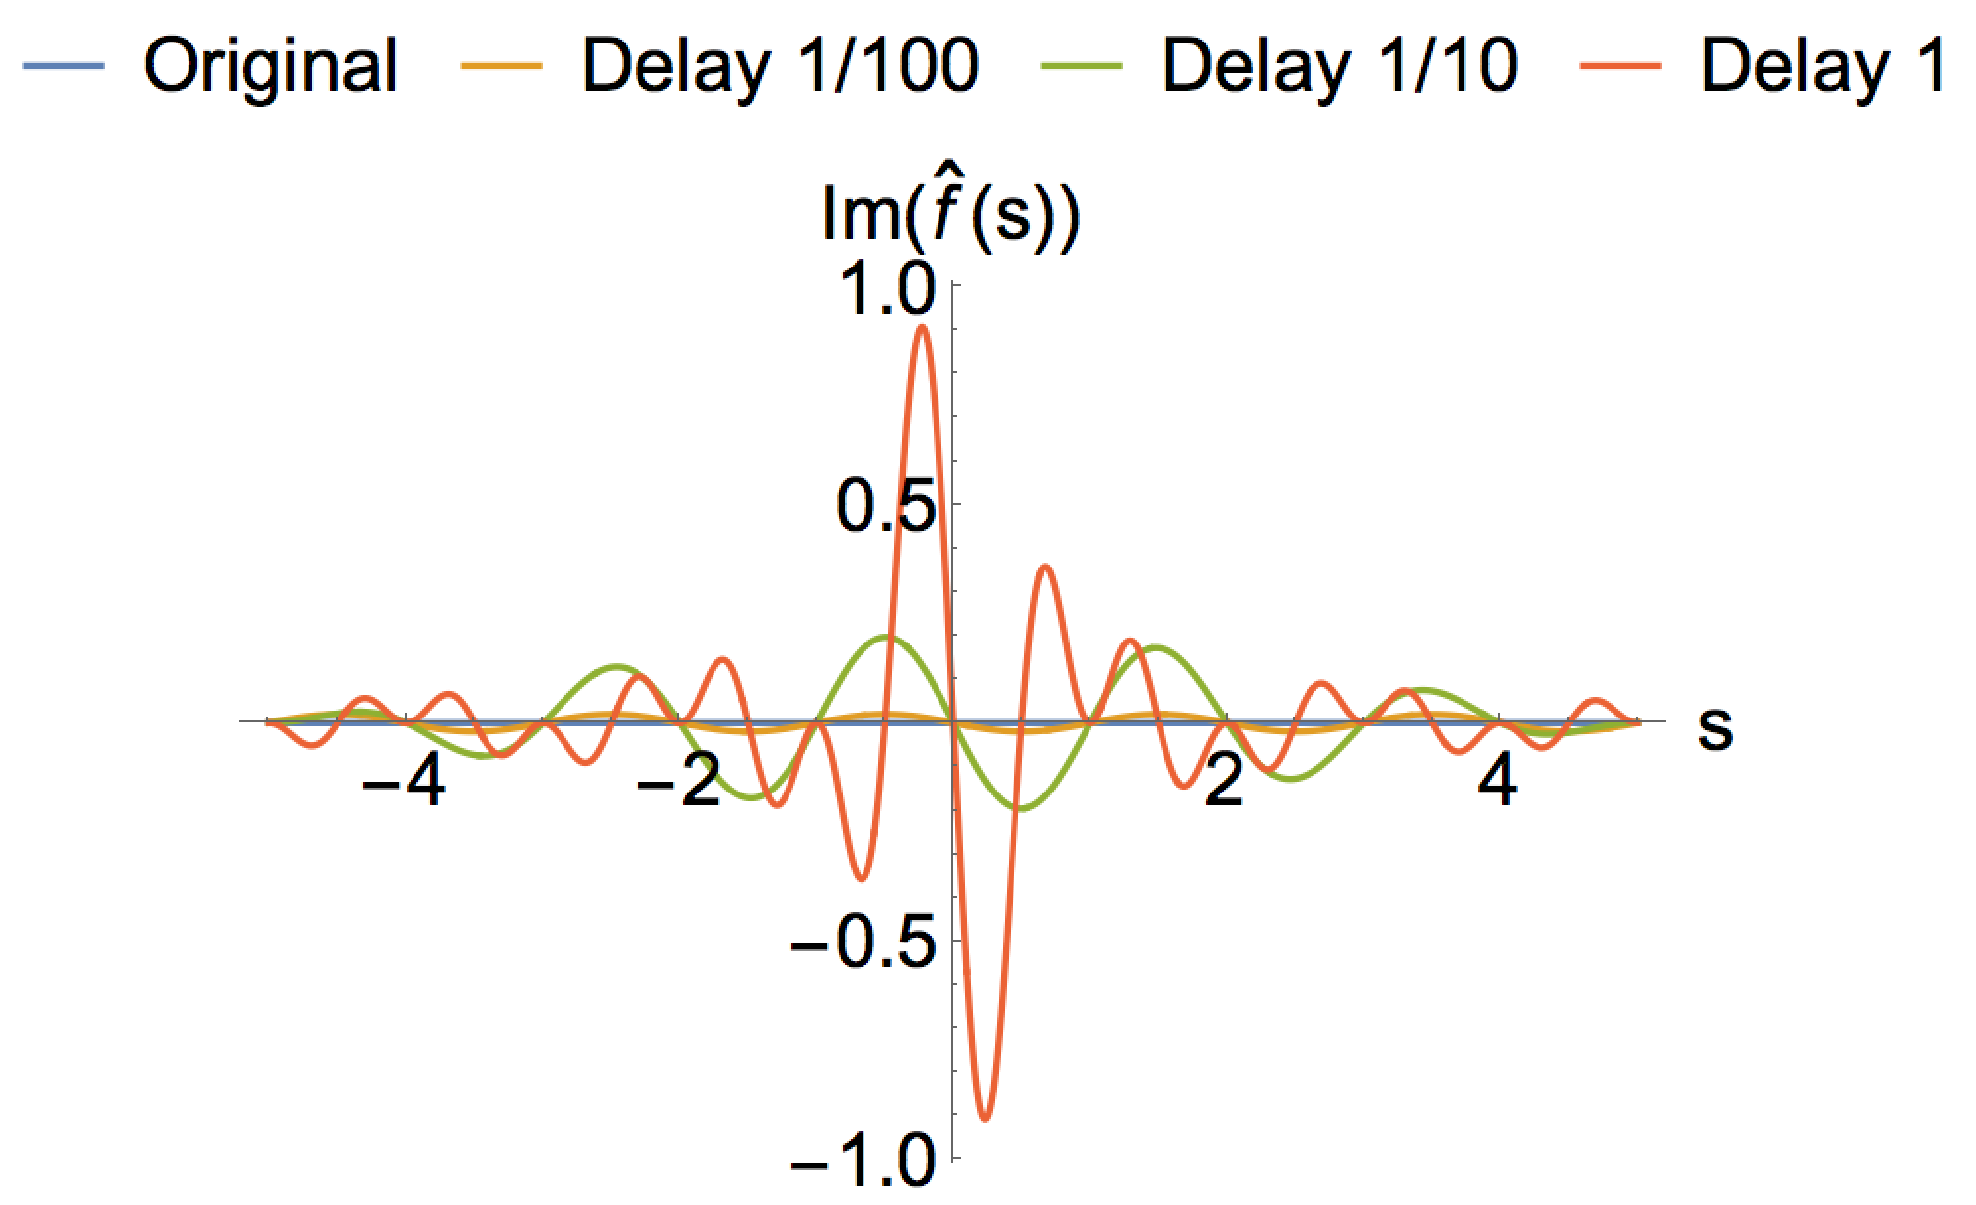
\includegraphics[scale=0.5]{tophatdelayim.png}
\end{tabular}

\subsection*{Solution}
2. You should find that $\hat{f}(s=2.9) = 0.0274405 + 0.0199367i$




%%%%%%%%%%%%%%%%%%%%%%%%%%%%%%%%%
\newpage
%%%%%%%%%%%%%%%%%%%%%%%%%%%%%%%%%
\section{Fourier transform of a stretched triangle function}

\subsection*{Resources}
\begin{itemize}
    \item Book: Chapter 2.2.8 (\url{https://see.stanford.edu/materials/lsoftaee261/book-fall-07.pdf})
    \item Video lecture 8 from 12:12 to 28:50 (\url{https://youtu.be/wUT1huREHJM?t=12m12s})
\end{itemize}

\subsection*{Challenge}
Since this can be a little confusing, please be sure to fully read the listed resource and make sure you understand the reasoning and derivation.

A triangle function of general width can be defined as

\begin{equation}
    f(at)=
    \begin{cases}
        1 - a|t| & \text{for } a|t| < 1\\
        0 & \text{otherwise}
    \end{cases}
\end{equation}

1. In challenge \ref{sec:ft_triangle} the base-width of the triangle was $2$ (ie, $1-(-1)$) and the half-base-width was $1$ (ie, $1-0$). What is the half-base-width for a triangle when $a=2$ and $a=1/2$?

2. Calculate the Fourier Transform $\hat{f}(s)$ for the case where the width of the triangle-function is doubled.

3. Write a few sentences explaining how stretching and squeezing in the time-domain is related to stretching and squeezing in the frequency domain.

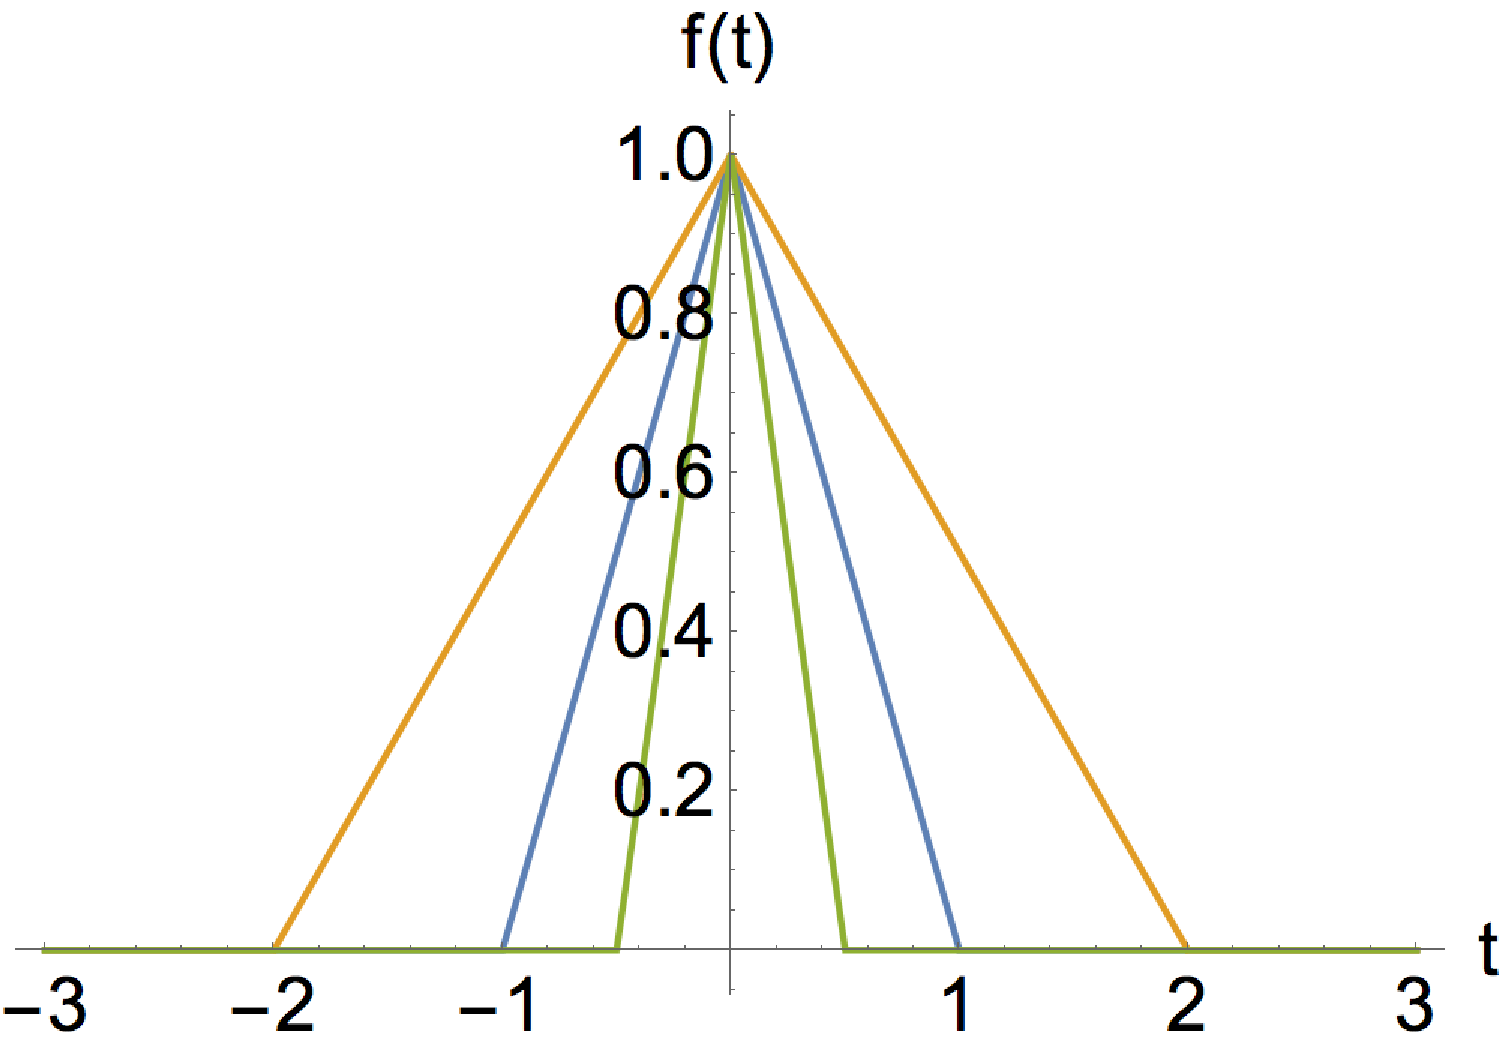
\includegraphics[scale=0.75]{triangledouble.png}

\subsection*{Solution}
1.\\
$\bm{a=2}$\\
\soltwodp{g}{3cd169}

$\bm{a=1/2}$\\
\soltwodp{h}{3bb5c8}

2.\\
To check your answer, evaluate the transform at $s=0.1$.\\
$\hat{f}(0.1)=1.75$




%%%%%%%%%%%%%%%%%%%%%%%%%%%%%%%%%
\newpage
%%%%%%%%%%%%%%%%%%%%%%%%%%%%%%%%%
\section{Fourier transform of a shifted-stretched function}
\label{sec:shiftstretch}

\subsection*{Resources}
\begin{itemize}
    \item Book: Chapter 2.2.9 (\url{https://see.stanford.edu/materials/lsoftaee261/book-fall-07.pdf})
\end{itemize}

\subsection*{Challenge}
Calculate the Fourier transform of the signal shown below.

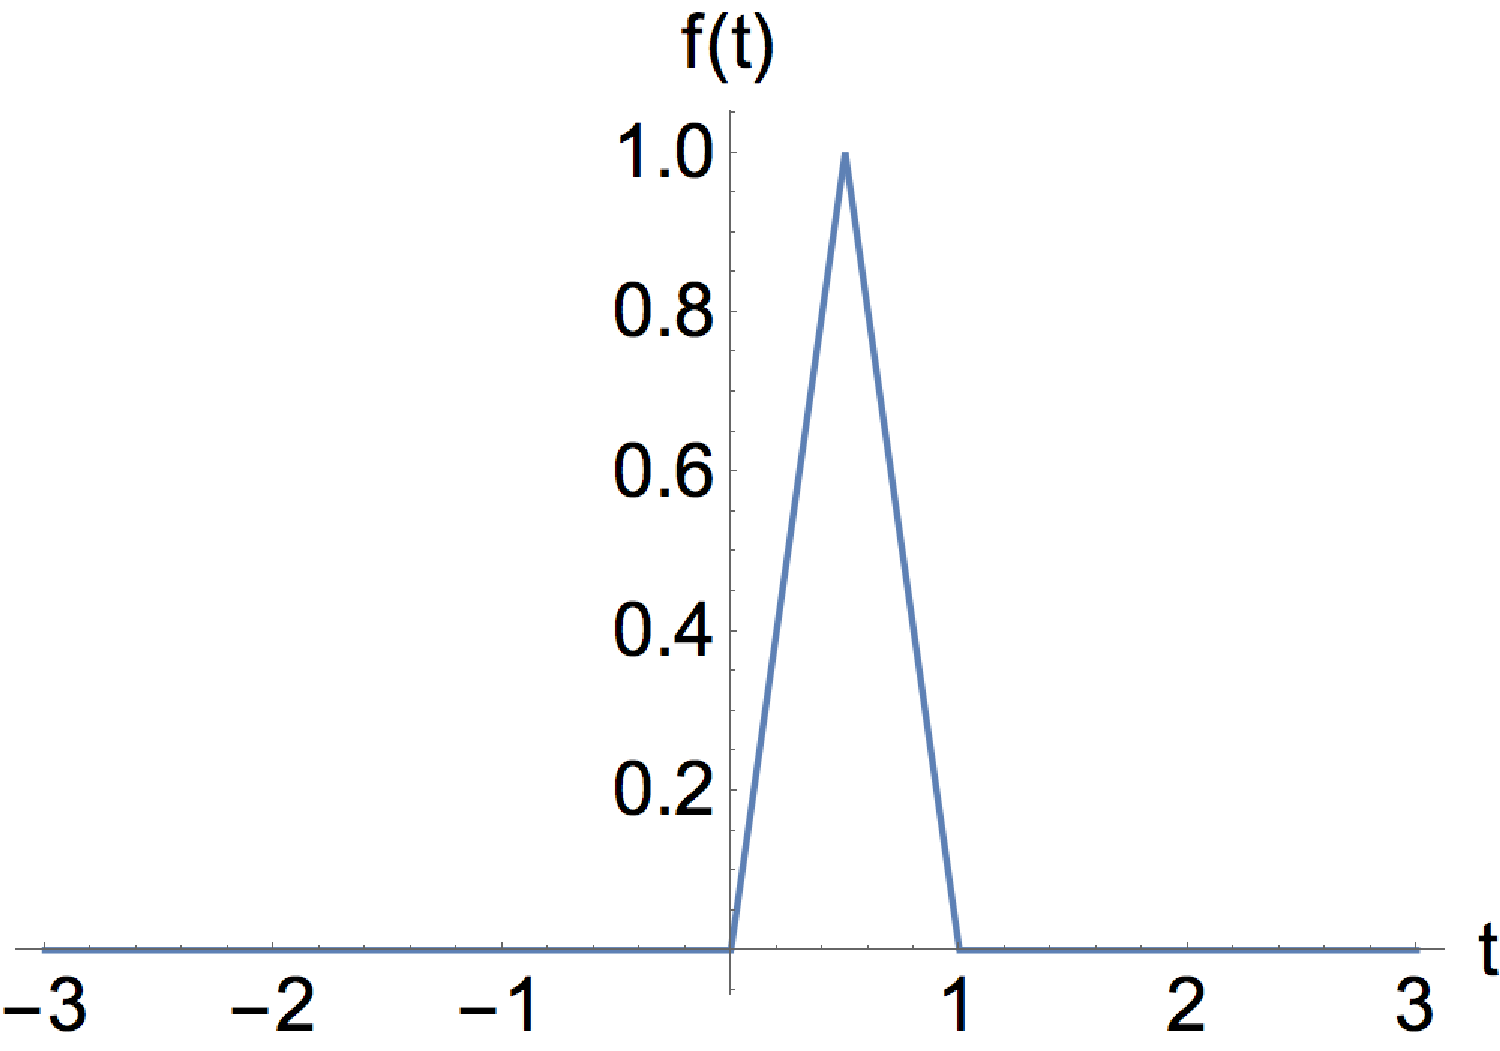
\includegraphics[width=8cm]{triangleshiftsqueeze.png}

\subsection*{Solution}
Your answer should be consistent with $\hat{f}(s=1.1) = -0.155 + 0.050 i$.



%%%%%%%%%%%%%%%%%%%%%%%%%%%%%%%%%
\newpage
%%%%%%%%%%%%%%%%%%%%%%%%%%%%%%%%%
\section{Convolution introduction}

\subsection*{Resources}
\begin{itemize}
    \item Video lecture 8 starting at 32:15: \url{https://youtu.be/wUT1huREHJM?t=32m15s}
\end{itemize}

\subsection*{Comment}
Here we expand our study to convolution; a powerful function for processing signals. Convolution is not immediately intuetive, but Prof. Osgood provides an excellent introduction.

\subsection*{Challenge}
Make notes following the above video deriving the formula relating convolution in the frequency and time domains.




%%%%%%%%%%%%%%%%%%%%%%%%%%%%%%%%%
\newpage
%%%%%%%%%%%%%%%%%%%%%%%%%%%%%%%%%
\section{Filtering}

\subsection*{Resources}
\begin{itemize}
    \item Video lecture 9 until 24:15: \url{https://www.youtube.com/watch?v=NrOR2qMVWOs}
\end{itemize}

\subsection*{Comment}
The above video includes an excellent example of using fourier analysis in a scientific context, including its application in filters.

The challenge below asks you to watch to 24:15, however after this point he goes on to describe the futility of trying to visualise convolution in the time-domain. Nevertheless, the graphics on convolution on Wikipedia [1] (especially these: [2a,b]) I think go some way to visualising what's happening in the time-domain.

1: \url{https://en.wikipedia.org/wiki/Convolution}\\
2a: \url{https://en.wikipedia.org/wiki/Convolution\#/media/File:Convolution_of_box_signal_with_itself2.gif}\\
2b: \url{https://en.wikipedia.org/wiki/Convolution\#/media/File:Convolution_of_spiky_function_with_box2.gif}

For your reference, turbidity standards of 5, 50, and 500 Nephelometric Turbidity Units (left to right respectively) are shown here:\\
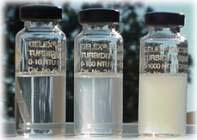
\includegraphics{turbidity.png}\\
\emph{Source: \url{https://en.wikipedia.org/wiki/Turbidity}}

\subsection*{Challenge}
1. Take notes following the above video until 24:15. There is a lot of useful information here. The questions below highlight the key points that I want you to understand, however they do not cover everything, so please be sure to follow the video.

2. Using a few sentences and diagrams, describe an ideal low-pass, high-pass and band-pass filter. How can they be applied in the frequency domain to influence the signal in the time-domain?

3. Write a few sentences and equations describing how convolution in the time-domain is related to signal multiplication in the frequency-domain.


%%%%%%%%%%%%%%%%%%%%%%%%%%%%%%%%%
\newpage
%%%%%%%%%%%%%%%%%%%%%%%%%%%%%%%%%
\section{Convolution with a window function}

\subsection*{Comment}
The ``signal'' here is $g(t-\tau)$ and the ``window function'' is $f(\tau)$.

\subsection*{Challenge}
1. Consider that you have a (somewhat unrealistic but mathematically manageable) input signal that varies as $g(t-\tau)=(t-\tau)^2$ with time. 

Obtain the convolution of the signal $(f \star g)(t)$ with a window function:
\begin{equation}
    f(\tau)=
    \begin{cases}
        1 & \text{for } -1/2 < \tau < 1/2\\
        0 & \text{otherwise}
    \end{cases}
\end{equation}

2. Compare the answer above when $t=0$ with direct integration of $\tau^2$ between $-1/2$ and $1/2$. Why are they the same?

\subsection*{Solution}
\hash{ppp}{290253}




%%%%%%%%%%%%%%%%%%%%%%%%%%%%%%%%%%
%\newpage
%%%%%%%%%%%%%%%%%%%%%%%%%%%%%%%%%%
%\section{Convolution with a continuous function}
%
%\subsection*{Challenge}
%Consider that you have a (somewhat unrealistic but mathematically manageable) input signal that varies with time $\tau$ as $f(\tau)=\tau$.  Apply a filter to the signal that is defined at time $t$ as $e^{-|t|}$.
%
%\emph{Hint: $\int_{-\infty}^{\infty} \text{(even function)} = 2 \int_{0}^{\infty} \text{(even function)}$.}
%
%To check your answer, substitute $t=1$ into your final answer.
%
%\subsection*{Solution}
%\hash{qqq}{e48f28}




%%%%%%%%%%%%%%%%%%%%%%%%%%%%%%%%%%
%\newpage
%%%%%%%%%%%%%%%%%%%%%%%%%%%%%%%%%%
%\section{Inequalities}
%
%\subsection*{Challenge}
%1. Re-write $-1/2 < t - \tau$ in the form $f(\tau) < t$ replacing $f(\tau)$ with appropriate expressions.
%
%2. Re-write $t - \tau < 1/2$ in the form $t < f(\tau)$ replacing $f(\tau)$ with appropriate expressions.
%
%3. Re-write $-1/2 < t - \tau < 1/2$ in the form $f(\tau) < t < g(\tau)$ replacing $f(\tau)$ and $g(\tau)$ with appropriate expressions.
%
%\subsection*{Solution}
%To check your solutions, substitute $\tau=1/2$ into the final expressions:
%
%1. $f(1/2)$: \hash{kkk}{115edb}\\
%2. $f(1/2)$: \hash{mmm}{6d64cd}\\
%3. $f(1/2)$: \hash{nnn}{414d80} and $g(1/2)$: \hash{ooo}{3ec4d7}




%%%%%%%%%%%%%%%%%%%%%%%%%%%%%%%%%%
%\newpage
%%%%%%%%%%%%%%%%%%%%%%%%%%%%%%%%%%
%\section{Touching window functions}
%\label{sec:touchingwindows}
%
%\subsection*{Challenge}
%1. Consider two window functions $f$ and $g$.
%\begin{equation}
%    f(\tau)=
%    \begin{cases}
%        1 & \text{for } -1/2 < \tau < 1/2\\
%        0 & \text{otherwise}
%    \end{cases}
%\end{equation}
%\begin{equation}
%    g(t-\tau)=
%    \begin{cases}
%        1 & \text{for } -1/2 < t-\tau < 1/2\\
%        0 & \text{otherwise}
%    \end{cases}
%\end{equation}
%You can imagine a fixed window function $f$ and a shiftable window-function $g$ (depending on the value of $t$). What is the value of $t$ in the following situations?
%
%a) The left side of window $f$ and the right side of window $g$ are touching.\\
%b) Complete overlap of windows $f$ and $g$.\\
%c) The right side of window $f$ and the left side of window $g$ are touching.
%
%2.\\
%a) Write a function that describes the position of the left-hand-side of window function $g$ at time $t$.\\
%b) Write a function that describes the position of the right-hand-side of window function $g$ at time $t$.\\
%To check your answers, substitute $t=1$ into your expressions.
%
%\subsection*{Solution}
%1.a) \hash{rrr}{1e3803}\\
%1.b) \hash{sss}{171271}\\
%1.c) \hash{ttt}{95acc3}\\
%
%2.a) \hash{uuu}{e27eca}\\
%2.b) \hash{vvv}{23da5b}




%%%%%%%%%%%%%%%%%%%%%%%%%%%%%%%%%
\newpage
%%%%%%%%%%%%%%%%%%%%%%%%%%%%%%%%%
\section{Convolution of two window functions}

\subsection*{Challenge}
%1. Show that the convolution of the two window functions in challenge \ref{sec:touchingwindows} in the time-domain results in the triangle function
%\begin{equation}
%    h(t)=
%    \begin{cases}
%        1+t & \text{for } 1 < t < 0\\
%        1-t & \text{for } 0 < t < 1\\
%        0 & \text{otherwise}
%    \end{cases}
%\end{equation}

In challenge \ref{sec:tophat} you calculated the spectrum of a window function. Imagine here you have two window functions $f(t)$ and $g(\tau)$.

\begin{equation}
    f(t)=
    \begin{cases}
        1 & \text{for } |t| < 1/2 \\
        0 & \text{for } |t| > 1/2
    \end{cases}
\end{equation}

\begin{equation}
    g(\tau)=
    \begin{cases}
        1 & \text{for } |\tau| < 1/2 \\
        0 & \text{for } |\tau| > 1/2
    \end{cases}
\end{equation}

1. Use your knowledge of the window-function in the frequency domain from challenge \ref{sec:tophat} to calculate the frequency-domain spectrum of the convolution of the two window functions.

2. Compare your answer to that obtained in challenge \ref{sec:ft_triangle}. What is the resulting function in the time-domain? \emph{This should be possible by comparison, without calculation.}

\subsection*{Solution}
To check your answer, substitute $s=1$ into your answers

1. 0.71

2. \hash{www}{9a90c0}


% Discrete (L19-10:30,L20)



% Calculate fourier transform of dirichlet window https://www.youtube.com/watch?annotation_id=annotation_655167&feature=iv&src_vid=8JKb9UN6W4c&v=_HJH3MekMHY
